% vim: fileencoding=utf-8:tw=0:noexpandtab:ts=4:sw=4
% -*- coding: utf-8 -*-

\documentclass[letterpaper, 10pt, conference]{ieeeconf}

\IEEEoverridecommandlockouts
\overrideIEEEmargins   

% packages
\usepackage[mathletters]{ucs}
\usepackage[utf8x]{inputenc}
\usepackage{graphicx}
\usepackage{microtype}
\usepackage{amsmath}
\usepackage{url}

% options
\graphicspath{{figures/}{generated-figures/}}

% commands
\newcommand{\fig}[1]{Figure~\ref{fig:#1}}
\newcommand{\Fig}[1]{Figure~\ref{fig:#1}}
\newcommand{\tbl}[1]{{Table}~\ref{fig:#1}}
\newcommand{\Tbl}[1]{{Table}~\ref{fig:#1}}
\newcommand{\sect}[1]{Section~\ref{sec:#1}}
\newcommand{\Sect}[1]{Section~\ref{sec:#1}}
\newcommand{\hypo}[1]{Hypothesis~\ref{hyp:#1}}
\newcommand{\Hypo}[1]{Hypothesis~\ref{hyp:#1}}
\newcommand{\algo}[1]{Algorithm~\ref{algo:#1}}
\newcommand{\Algo}[1]{Algorithm~\ref{algo:#1}}
\newcommand{\eq}[1]{Equation~\ref{eq:#1}}
\newcommand{\Eq}[1]{Equation~\ref{eq:#1}}

% title and authors

\title{\LARGE \bf
Localization of inexpensive robots with low-bandwidth sensors
}

\author{Shiling Wang$^{1}$ and Francis Colas$^{2}$ and Ming Liu$^{3}$ and Francesco Mondada$^{4}$ and Stéphane Magnenat$^{5}$% <-this % stops a space
\thanks{$^{1}$Shiling Wang is with ETH Zürich
        {\tt\small shilingwang0621@gmail.com}}%
\thanks{$^{2}$Fraucis Colas is with INRIA Nancy Grand Est
        {\tt\small francis.colas@inria.fr}}%
\thanks{$^{3}$Ming Liu is with City University of Hong Kong
        {\tt\small mingliu@cityu.edu.hk}}%
\thanks{$^{4}$Francesco Mondada is with Mobots, LSRO, EPFL
        {\tt\small francesco.mondada@epfl.ch}}%
\thanks{$^{5}$Stéphane Magnenat is with Mobots, LSRO, EPFL
        {\tt\small stephane@magnenat.net}}%
}

\begin{document}

\maketitle
\thispagestyle{empty}
\pagestyle{empty}

\begin{abstract}
Lorem ipsum...
\end{abstract}

\section{Introduction}

Why localisation is useful for cheap robot in educational context, why it is not trivial?

Highlight challenges



\section{Related work}

Markov and Monte Carlo Localization, why not SLAM?

Localization techniques for cheap mobile robots.

\section{Material}

\subsection{Thymio robot}

Thymio and Aseba~\cite{magnenat2012arso, aseba2011tmech, riedo2013arso}.

\subsection{Map}

\subsection{Data acquisition}

\section{Model}

\subsection{Variables}

The model uses the following variables:
\begin{itemize}
\item $X_{1:t}$ 2-D pose at times $1..t$.
The pose vector consists of $x,y$ coordinates and an angle $\theta$.
\item $Z_{1:t}$ observations at times $1..t$.
The observation consists of two sensors located at the bottom of the robot, measuring the intensity of the ground.
\item $U_{1:t}$ odometry at times $1..t$.
The odometry consists of the left and right wheel speeds.
\end{itemize}

\subsection{Constants}

The following constants are parameters of the model:
\begin{itemize}
\item $\alpha_\mathrm{xy}$ the std. dev. of the motion model in translation
\item $\alpha_\theta$ the std. dev. of the motion model in rotation
\item $p_\mathrm{uniform}$ ratio of uniform probabilty added at observation time to represent kidnapping
\item $\sigma_{obs}$ the std. dev. of the grayscale intensity in the observation model
\end{itemize}
The first three constants are found using maximum likelyhood (see \sect{mle}), the last one is selected based on the knowledge of the sensor.

\subsection{Joint probability}

The joint probability is:
\begin{equation}
\begin{split}
& p(X_{1:t}, Z_{1:t}, U_{1:t}) = \\
& p(Z_t|X_t) p(X_t|X_{t-1}, U_{t}) p(U_t) p(X_{1:t-1}, Z_{1:t-1}, U_{1:t-1})
\end{split}
\end{equation}

\subsection{Question}

We want to estimate the pose $X_t$ at time $t$ knowing the observations $Z_{1:t}$ and the commands $U_{1:t}$, using a recursive filter:
\begin{equation}
\begin{split}
& p(X_t|Z_{1:t},U_{1:t}) = \frac{p(X_t,Z_t | Z_{1:t-1}, U_{1:t})}{p(Z_t|Z_{1:t-1}, U_{1:t})} \\
 &\propto p(Z_t | X_t) p(X_t | Z_{1:t-1}, U_{1:t}) \\
 &\propto p(Z_t | X_t) \sum_{X_{t-1}} p(X_t, X_{t-1} | Z_{1:t-1}, U_{1:t} ) \\
 &\propto p(Z_t | X_t) \sum_{X_{t-1}} p(X_t|X_{t-1}, U_t) p(X_{t-1} | Z_{1:t-1}, U_{1:t-1})
\end{split}
\end{equation}
%This is a recursive filter to estimate $X_t$ using the previous estimation $X_{t-1}$, the odometry $U_t$ and the observation $Z_t$.

\subsection{Distributions}

\subsection{Markov implementation}

% TODO: talk about max_prob_error

\subsection{Monte Carlo implementation}

\subsection{Theoretical analysis}
% TODO place at correct place
% TODO text could be adapted, some equations removed, etc. in case it's too long.
For the aim of localizing a robot in a given know space, we can get an idea of the time required to be localized.
For the Markov Localization approach, we can see that there is a given number of discrete cells.
The amount of information needed to unambiguously specify one among them all is:
\begin{displaymath}
	H_{loc} = \log_2(N_cells) = \log_2\left(\frac{L\times W\times N_{\theta}}{h^2}\right),
\end{displaymath}
with $N_cells$ the number of cells, $L$ and $W$ the length and width of the environment, $h$ the size of the cell, and $N_{\theta}$ the number of discretization steps of the angle $\theta$ of the robot.
In our example with a 1.5\,m$\times$1.5\,m environment discretized with cells of 1\,cm and 5° angle, the amount of information needed for the localization is around 20.6 bits.

A binary sensor ideally yields 1 bit of information per measurement.
However in practice, there is a loss in information due to the sensor noise, characterized above with the $p_{\mbox{correct}}$ probability of the sensor to be correct:
\begin{displaymath}
	H_{noise} = H_{\mbox{b}}(1 - p_{\mbox{correct}}),
\end{displaymath}
where $H_{\mbox{b}}$ is the binary entropy function: $H_{\mbox{b}}(p) = -p\log_2(p) - (1-p)\log_2(1-p)$.
With $p_{\mbox{correct}}=0.95$ the loss in information is around 0.29 bit per measurement.

In addition to the noise, we need to take into account that our sensor measurements are not completely independent.
For example, when not moving, we observe always the same place and thus cannot really gain additional information besides being sure of the color of the current pixel.
In a discretized world, we thus need to estimate the probability of having changed cell in order to observe something new, which depends on the distance travelled and the size of the cells.
This problem is equivalent to the Buffon-Laplace needle problem of finding the probability for a needle thrown randomly on a grid to actually intersect the grid.\footnote{\url{http://mathworld.wolfram.com/Buffon-LaplaceNeedleProblem.html}}
In our case, the probability of not changing cell is given by:
\begin{displaymath}
	p_{\mbox{same}} = \frac{4d h - d^2}{\pi h^2},
\end{displaymath}
with $d$ the distance travelled.

We can then compute the conditional entropy for two successive ideal measurements separated by $d$:
\begin{displaymath}
	H(O_t | O_{t-1}) = H(O_t, O_{t-1}) - H(O_{t-1}).
	% That's a really generic formula, but giving the 2x2 matrix or the expression with the logs is probably too much
\end{displaymath}
With a robot moving at around 3\,cm/s with a timestep of 0.3\,s with 3\,cm cells, we have $d=0.9$\,cm and the loss of information due to the redundancy of around 0.33 bit.

The computation is similar with a second sensor placed on the robot.
The probability that they see the same cell based on the distance between them is exactly the same.
On our small robots, the sensors are 2.2\,cm apart so their redundancy causes a loss of information of 0.041 bit.

If we combine all these effects, we can bound the information that our robot gathers at each timestep to at most 1.05 bit and a time to localize of at least 6\,s.
In order to have a faster localization, the greatest changes could be to move faster, in order to reduce redundancy in the successive measurements, or to have better sensors.
Setting the sensors apart also reduces the redundancy between their information but given our grid size, they are sufficiently separated.

\subsection{Dataset collection}

\subsection{Parameter estimation}
\label{sec:mle}

\section{Results}

\subsection{Basic localization}

\begin{figure*}

\begin{center}
Markov Localization, run \emph{random\_1}
\end{center}
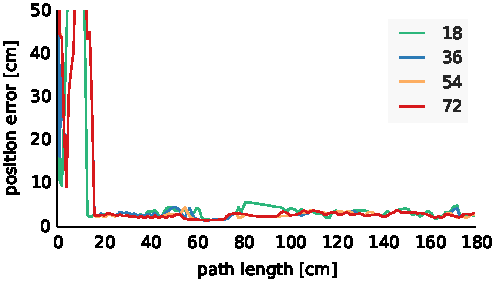
\includegraphics{ml-whole_random_1-xy}\hfill
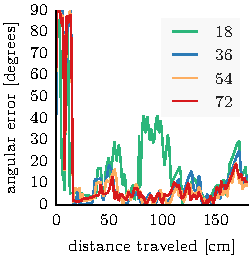
\includegraphics{ml-whole_random_1-theta}

\vspace{.5em}

\begin{center}
Markov Localization, run \emph{random\_2}
\end{center}
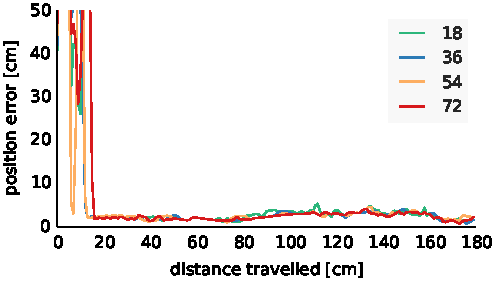
\includegraphics{ml-whole_random_2-xy}\hfill
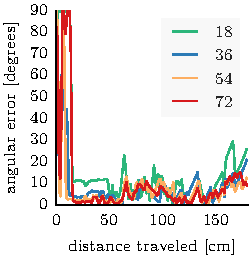
\includegraphics{ml-whole_random_2-theta}

\vspace{.5em}

\begin{center}
Monte Carlo Localization, run \emph{random\_1}
\end{center}
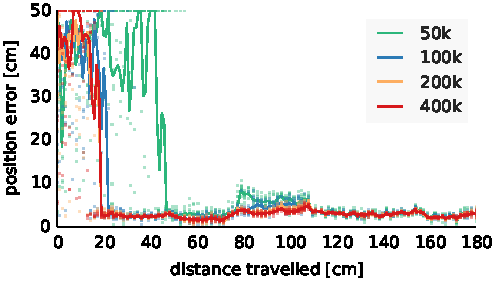
\includegraphics{mcl-whole_random_1-xy}\hfill
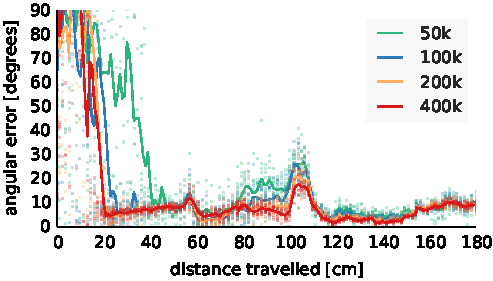
\includegraphics{mcl-whole_random_1-theta}

\vspace{.5em}

\begin{center}
Monte Carlo Localization, run \emph{random\_2}
\end{center}
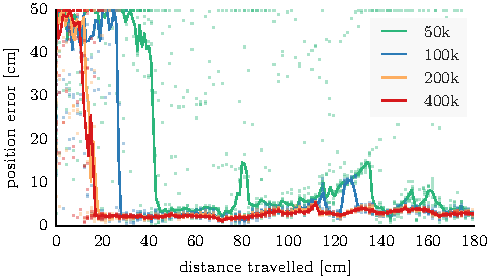
\includegraphics{mcl-whole_random_2-xy}\hfill
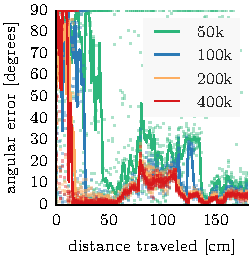
\includegraphics{mcl-whole_random_2-theta}

\caption{The error in position and orientation between the estimation by the localization algorithm and the ground truth, using Markov and Monte Carlo localization, on two runs.
For Markov localization, the legend indicates the number of discretization steps for angles; for Monte Carlo localization, it indicates the number of particles.
For Monte Carlo localization, the solid lines show the average over 10 trials, while the light dots show the individual trials.
The error is clamped at 50\,cm for position and 90° for orientation.}
\label{fig:whole-runs-random12}
\end{figure*}

\Fig{whole-runs-random12} shows the error in position and orientation for runs \emph{random\_1} and \emph{random\_2}.
In these plots, \emph{path length} represents the cumulative distance travelled by the center point between the two ground sensors of the robot.

For Markov localization, all discretization resolutions allow the robot to localize with a precision of 3\,cm and 5°.
In run \emph{random\_1}, the resolution of 18 is not enough to keep tracking the orientation at path lengths 50\,cm and 80\,cm.
These both correspond to the robot rotating on spot.
We see that a discretization of 36 (10° resolution) is sufficient to provide accurate tracking, and that a finer resolution only provides minor improvements in angular precision, and no improvement in position precision.
In run \emph{random\_3}, we see that a resolution of 54 is allows for a better angular precision than 36, but 72 does not improves over 54.
All resolutions provide equal position precision.

For Monte Carlo localization, we see that on run \emph{random\_1}, the robot localizes already with 50k particles, but twice later than with 100k particles.
Increasing the number of particles over this value only provides minor decrease in localization time and precision.
While 50k particles allow to localize on this run in average, there are some trials (restart of the run) in which the robot looses orientation, when it turns on spot.
On run \emph{random\_2}, 50k particles is not enough for localizing the robot.
Increasing this number to 100k leads to a good localization, exception during path lengths 80--100; indeed this corresponds to a long moment during which the robot rotates on spot, leading to less information acquisition, and therefore degradated precision.
%TODO: explain why this does not appear in ML

\subsection{Robot kidnapping}

\begin{figure*}

\begin{center}
Markov Localization, run \emph{random\_long}
\end{center}
%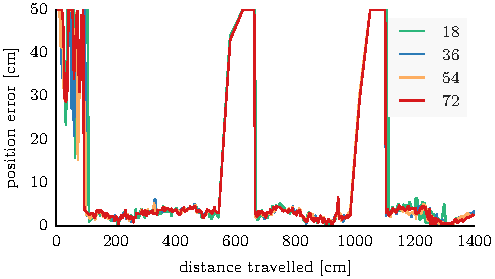
\includegraphics{ml-whole_random_long-xy}\hfill
%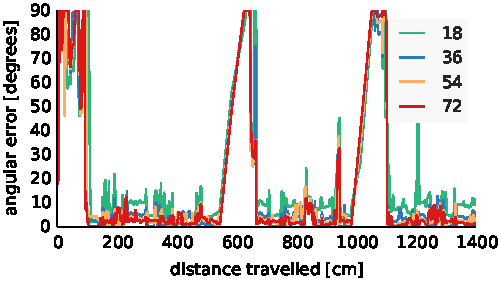
\includegraphics{ml-whole_random_long-theta}

\vspace{.5em}

\begin{center}
Monte Carlo Localization, run \emph{random\_long}
\end{center}
%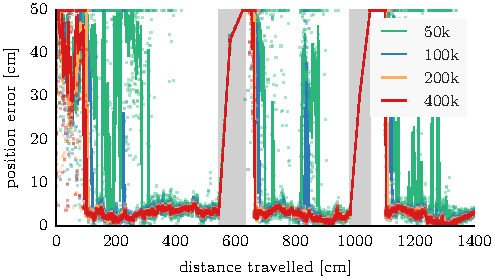
\includegraphics{mcl-whole_random_long-xy}\hfill
%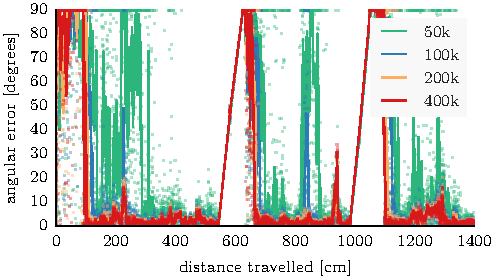
\includegraphics{mcl-whole_random_long-theta}

\caption{The error in position and orientation between the estimation by the localization algorithm and the ground truth, using Markov and Monte Carlo localization, on the run with kidnapping.
For Markov localization, the legend indicates the number of discretization steps for angles; for Monte Carlo localization, it indicates the number of particles.
For Monte Carlo localization, the solid lines show the average over 10 trials, while the light dots show the individual trials.
The error is clamped at 50\,cm for position and 90° for orientation.}
\label{fig:whole-runs-random-long}
\end{figure*}

\Fig{whole-runs-random-long} shows the error in position and orientation for the run with kidnapping.
In this run, the robot is kidnapped twice, at path length 550\,cm and 1000\,cm.
It takes the robot approximately 50\,cm to relocalize, and does so successfully with both Markov and Monte Carlo localization.
With Markov Localization, discretization resolutions of 54 and 72 are approximately equivalent in performance, while 36 and 18 perform clearly worst.
With Monte Carlo, the robot localizes most of the time with 100k particle or more, and always with 200k particles or more.
%TODO: reanalyse MCL once we have 10 runs

\begin{figure*}

\begin{center}
Markov Localization, average of 10 extracts from \emph{random\_1} and \emph{random\_2}
\end{center}
%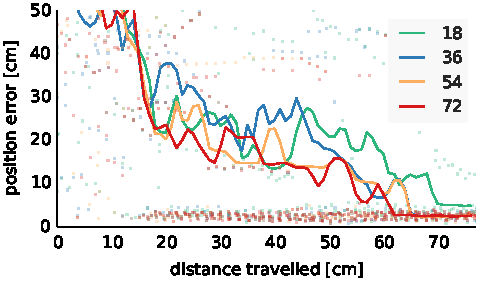
\includegraphics{ml-small_runs_random_12-xy}\hfill
%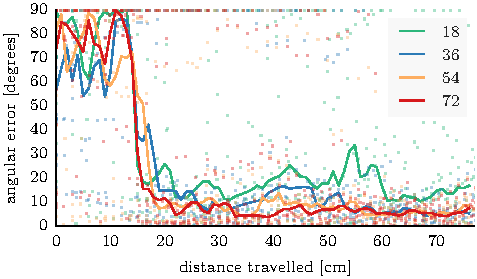
\includegraphics{ml-small_runs_random_12-theta}

\vspace{.5em}

\begin{center}
Monte Carlo Localization, average of 10 extracts from \emph{random\_1} and \emph{random\_2}
\end{center}
%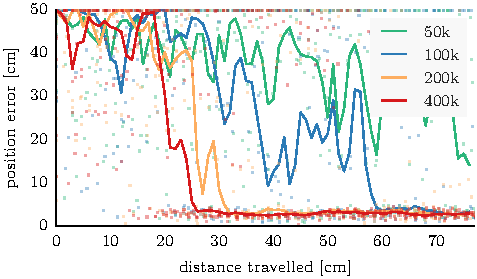
\includegraphics{mcl-small_runs_random_12-xy}\hfill
%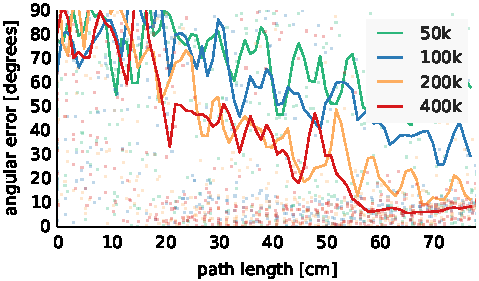
\includegraphics{mcl-small_runs_random_12-theta}

\caption{
The error in position and orientation between the estimation by the localization algorithm and the ground truth, using Markov and Monte Carlo localization, on 10 extracts from two runs.
For Markov localization, the legend indicates the number of discretization steps for angles; for Monte Carlo localization, it indicates the number of particles.
The solid lines show the average over 10 trials, while the light dots show the individual trials.
The error is clamped at 50\,cm for position and 90° for orientation.}
\label{fig:small-runs}
\end{figure*}

\subsection{Theoretical length to converge}

%TODO

\subsection{Real-time with Thymio}

\section{Discussion}

What works, what does not, why?

Why sampling-based approach is not so easy, but propose how it could be done.

\section{Conclusion}

This paper provides several contributions to the state of the art of localization of robots with low-bandwidth sensors:
\begin{itemize}
\item an empirical evaluation of Markov- and Monte Carlo-based implementations;
\item a predictive model allowing designers to select and place sensors to achieve a desired localization performance;
\item a process to let end-users create and provide their own environments, such as drawings made by children.
\end{itemize}
Together, these allow absolute positioning of educational mobile robots in the 100 Euro price range.
This opens many educational opportunities, such as the study of geometry, puzzles based on the physical space, and staging the creation of stories in the context of language education.
These new possibilities are key elements for robots to answer the need for embodied computational thinking education.

\bibliographystyle{IEEEtran}
\bibliography{thymio-localisation-icra}

\end{document}



